\documentclass{beamer}
\usefonttheme[onlymath]{serif}
\usepackage[T1]{fontenc}
\usepackage[utf8]{inputenc}
\usepackage[english, icelandic]{babel}
\usepackage{amsmath}
\usepackage{amssymb}
\usepackage{amsthm}
\usepackage{mathabx}
\usepackage{parskip}
\usepackage{mathtools}
\usepackage{multicol}

\renewcommand\Im{\operatorname{Im}}
\renewcommand\Re{\operatorname{Re}}

\title{Rudin-Carleson theorems}
\author{Bergur Snorrason}
\date{\today}

\begin{document}

\frame{\titlepage}

\begin{frame}
\begin{enumerate}
\item[$\cdot$] The focus of the thesis is the Rudin-Carleson theorem and its variations.
\item[$\cdot$] These theorems are what we call extension theorems, that is, they tell us when we can extend a function to a larger set while maintaining some properties.
\item[$\cdot$] Concretely, if $f \colon A \rightarrow X$, $g \colon B \rightarrow X$, $A \subset B$ and $f = g$ on $A$, then we say $g$ \emph{extends} $f$.
\end{enumerate}
\begin{multicols}{2}
\begin{enumerate}
\item[$\cdot$] We will use the following to denote common sets in $\mathbb{C}$.
\begin{enumerate}
\item[$\cdot$] $\mathbb{D} = \{z \in \mathbb{C} \colon |z| < 1\}$
\item[$\cdot$] $\overline{\mathbb{D}} = \{z \in \mathbb{C} \colon |z| \leq 1\}$
\item[$\cdot$] $\mathbb{T} = \{z \in \mathbb{C} \colon |z| = 1\}$
\end{enumerate}
\end{enumerate}
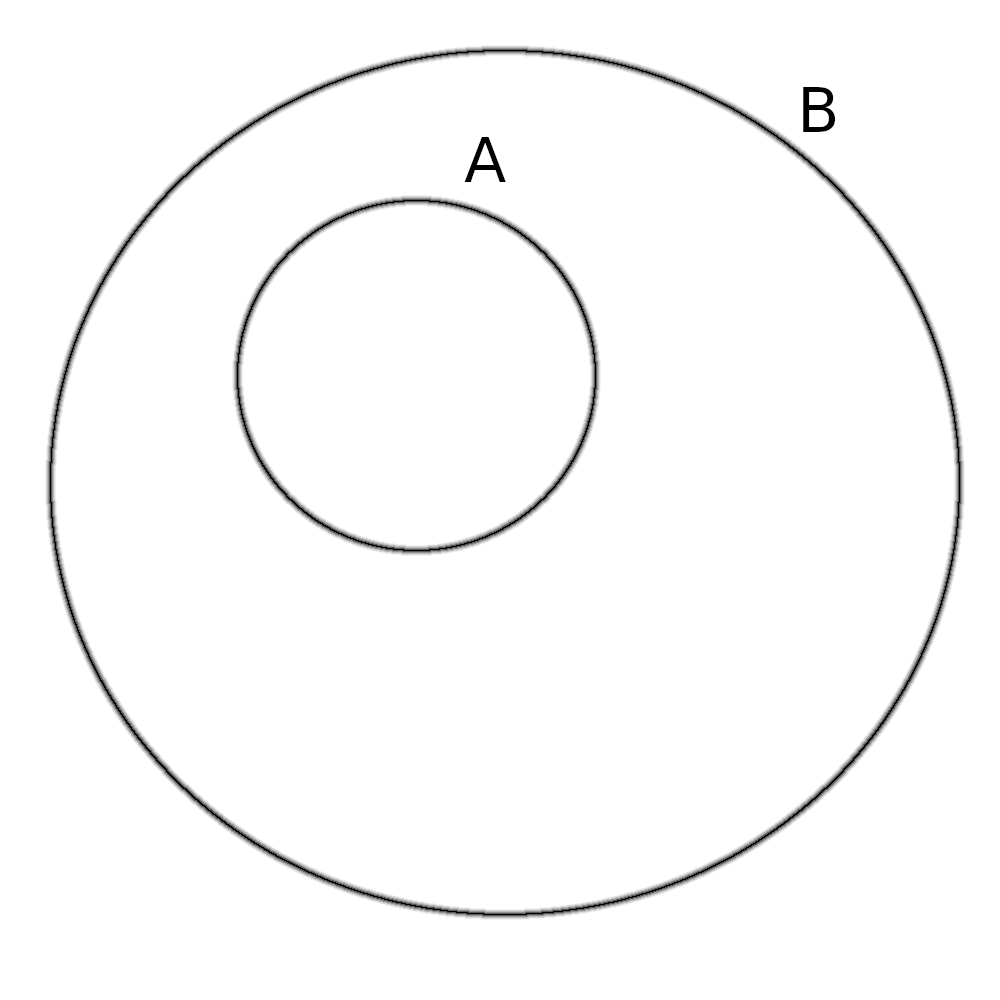
\includegraphics[width=0.3\textwidth]{extend}
\end{multicols}
\end{frame}

\begin{frame}
\begin{enumerate}
\item[$\cdot$] We will look at two famous examples of extension theorems before looking at the Rudin-Carleson theorem
\item[$\cdot$] The first one is Tietze's extension theorem, from topology.
\item[$\cdot$] We say a topological space is \emph{normal} if all disjoint closed sets can be separated by open neighbourhoods and if the singletons are closed. 
\begin{center}
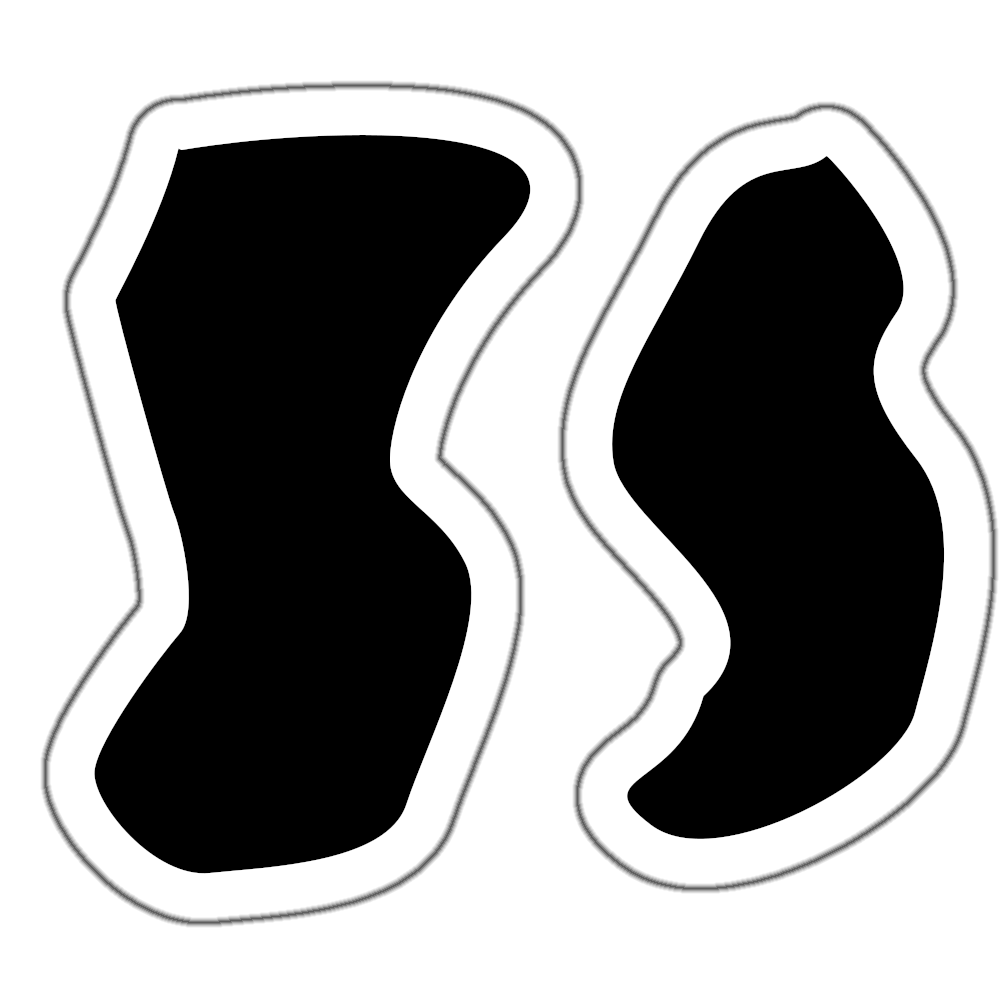
\includegraphics[width=0.3\textwidth]{normal}
\end{center}
\item[$\cdot$] All metric spaces are normal and so are compact Hausdorff spaces.
\end{enumerate}
\end{frame}

\begin{frame}
\begin{theorem}[Tietze]
Let $X$ be a normal space and $A$ be a closed subset of $X$.
For any continuous function $f \colon A \rightarrow \mathbb{R}$ there exists a $g \colon X \rightarrow \mathbb{R}$ that extends it.
\end{theorem}
\begin{theorem}[Tietze]
Let $X$ be a normal space and $A$ be a closed subset of $X$.
For any continuous function $f \colon A \rightarrow [a, b]$ there exists a $g \colon X \rightarrow [a, b]$ that extends it.
\end{theorem}
\end{frame}

%\begin{frame}
%\begin{theorem}[Carathéodory]
%If $\Omega_1$ and $\Omega_2$ are open subsets of $\mathbb{C}$ each bounded by a simple, closed curve and $f \colon \Omega_1 \rightarrow \Omega_2$ is a holomorphic bijection then there exists a continuous injection $g \colon \overline{\Omega_1} \rightarrow \overline{\Omega_2}$ that extends $f$.
%\end{theorem}
%\end{frame}

\begin{frame}
\begin{enumerate}
\item[$\cdot$] Recall that a function defined on an open subset of $\mathbb{C}$ is \emph{harmonic} if
\[
	\frac{\partial^2f}{\partial x^2} + \frac{\partial^2f}{\partial y^2} = 0.
\]
\item[$\cdot$] We define the \emph{Poisson kernel} on $\mathbb{D}$ by
\[
	P(z, e^{it}) = \frac{1 - |z|^2}{|e^{it} - z|^2}.
\]
\item[$\cdot$] If $f$ is an integrable function defined on $\mathbb{T}$ then we define its \emph{Poisson integral} by
\[
	P[f](z) = \frac{1}{2\pi} \int_{-\pi}^{\pi} P(z, e^{it})f(e^{it})\ dt.
\]
\end{enumerate}
\end{frame}

\begin{frame}
\begin{enumerate}
\item[$\cdot$] Given a continuous function $f$ on the unit circle $\mathbb{T}$ can you find a continuous function $u$ on $\overline{\mathbb{D}}$ that's harmonic on $\mathbb{D}$ and agrees with $f$ on $\mathbb{T}$.
\item[$\cdot$] This is the famous Dirichlet problem on the unit disk.
\item[$\cdot$] We can define such a $u$ by
\[
	u(z) = \left \{
	\begin{array}{l l}
		f(z), & |z| = 1\\
		P[f](z), & |z| < 1
	\end{array}
	\right .
\]
to solve this problem.
\item[$\cdot$] In other words, we can use the Poisson kernel to extend $f$ harmonically into $\mathbb{D}$.
\end{enumerate}
\end{frame}

\begin{frame}
\begin{enumerate}
\item[$\cdot$] The Dirichlet problem is about extending harmonically, but can we extend holomorphically?
\item[$\cdot$] The set of all continuous functions on the closed unit disk $\overline{\mathbb{D}}$ which are holomorphic on the open unit disk  $\mathbb{D}$ is called the \emph{disk algebra} and we denote it by $\mathcal{A}$.
\item[$\cdot$] A theorem from the study of Hardy spaces tells us that if a $f$ is a function in $\mathcal{A}$ and
\[
	m(\{z \in \mathbb{T} \colon f(z) = 0\}) > 0,
\]
where $m$ is the arc length measure on $\mathbb{T}$, then $f = 0$.
\item[$\cdot$] So not all continuous functions on the unit circle $\mathbb{T}$ can be extended to $\mathcal{A}$.
\item[$\cdot$] We can always extend, however, if we limit ourselves to a sufficiently small subset of $\mathbb{T}$.
\end{enumerate}
\end{frame}

\begin{frame}
\begin{theorem}[Rudin-Carleson (1956-1957)]
Let
	$E$ be a closed subset of $\mathbb{T}$ such that $m(E) = 0$,
	$f \colon E \rightarrow \mathbb{C}$ be continuous,
	and $T$ be a subset of $\mathbb{C}$ homeomorphic to $\overline{\mathbb{D}}$ such that $f(E) \subset T$.
There exists a function $g$ in $\mathcal{A}$ that extends $f$ and $g(\overline{\mathbb{D}}) \subset T$.
\end{theorem}
\end{frame}

\begin{frame}
\begin{enumerate}
\item[$\cdot$] This is proved twice in the thesis, first in the same manner Rudin did originally and then as consequence of Bishop's theorem and the F. and M. Riesz theorem.
\item[$\cdot$] Both of these proofs, at some point, use the Poisson integral solution of the Dirichlet problem mentioned earlier.
\item[$\cdot$] To discuss Bishop's theorem we first have to find a way to classify a set as sufficiently small (like $E$ in the Rudin-Carlson theorem) with regards to the family of functions we want to extend into.
\end{enumerate}
\end{frame}

\begin{frame}
\begin{enumerate}
\item[$\cdot$] Let $B$ be a family of measurable functions defined on $X$.
\item[$\cdot$] We say a measure $\mu$ is an \emph{annihilating measure of $B$} if
\[
	\int_X g\ d\mu = 0
\]
for all $g$ in $B$.
\item[$\cdot$] We denote by $B^{\perp}$ the family of all the annihilating measures of $B$.
\item[$\cdot$] A set $E$ is said to be $B^{\perp}$-null if it is $\mu$-null for all $\mu$ in $B^{\perp}$.
\item[$\cdot$] We can intuitively think of it like this: Increasing the size of $B$, means you have fewer annihilating measures, which leads to more $B^{\perp}$-null sets.
\end{enumerate}
\end{frame}

\begin{frame}
\begin{theorem}[Bishop (1962)]
Let
\begin{enumerate}
\item $X$ be a compact Hausdorff space,
\item $B$ be a closed subspace of $(C(X), \| \cdot \|_{\infty})$,
\item $S$ be a closed subset of $X$ that is $B^{\perp}$-null,
\item $f$ be a continuous function on $S$,
\item $\Psi: X \rightarrow [0, +\infty[$ be a continuous function such that $|f| < \Psi$ on $S$.
\end{enumerate}
Then there exists a function $F \in B$ that extends $f$ and $|F| < \Psi$ on $X$. \\
\end{theorem}
\end{frame}

\begin{frame}
\begin{enumerate}
\item[$\cdot$] To show that this is a generalized version of the Rudin-Carleson theorem we need a connection between the annihilating measures of $\mathcal{A}$ and the arc length measure on $\mathbb{T}$.
\item[$\cdot$] That is, if $E$ is a closed subset of $\mathbb{T}$ that is $m$-null and $\mu$ is an annihilating measure of $\mathcal{A}$ then we need to show that $E$ is also $\mu$-null.
\end{enumerate}
\end{frame}

\begin{frame}
\begin{theorem}[F. and M. Riesz (1916)]
Let $\mu$ be a measure on $\mathbb{T}$ such that
\[
	\int_{\mathbb{T}} e^{-int}\ d\mu(t) = 0
\]
holds for $n = -1, -2, ...$.
Then $\mu \lll m$.
That is, if $E \subset \mathbb{T}$ is $m$-null then $E$ is also $\mu$-null.\\
\vspace{1em}
% This in addition to Bishop's theorem implies Rudin-Carleson, since $z \mapsto z^n$ are entire, and therefore in $\mathcal{A}$ (when restricted to $\mathbb{D}$).
\end{theorem}
\end{frame}

\begin{frame}
\begin{enumerate}
\item[$\cdot$] Let's look at a few examples of how we can use Bishop's theorem.
\item[$\cdot$] Let $X = \mathbb{T}$, $B = \mathcal{A}$ and $E$ be a closed subset of $\mathbb{T}$ such that $m(E) = 0$.
\item[$\cdot$] If $\mu$ is in $B^{\perp}$ then it satisfies the condition of the F. and M. Riesz theorem so $E$ is $\mu$-null.
\item[$\cdot$] So $E$ is $B^{\perp}$-null.
\item[$\cdot$] Bishop's theorem then tells us that all continuous functions on $E$ can be extended with a function in $\mathcal{A}$. 
\end{enumerate}
\end{frame}

\begin{frame}
\begin{enumerate}
\item[$\cdot$] Let $B = C(X)$.
\item[$\cdot$] If $\mu$ is in $B^{\perp}$ then, as a consequence of the Riesz representation theorem, $\mu = 0$.
\item[$\cdot$] That is $\mu = 0$ is the only annihilating measure of $B$.
\item[$\cdot$] So all subsets of $X$ are $B^{\bot}$-null.
\item[$\cdot$] This result agrees with Tietze's extension theorem.
\end{enumerate}
\end{frame}

\begin{frame}
\begin{enumerate}
\item[$\cdot$] Let $B$ include only the zero function.
\item[$\cdot$] Then every measure is an annihilating measure of $B$.
\item[$\cdot$] Subsequently, no subset of $X$ is $B^{\perp}$-null, and Bishop's theorem gives us nothing.
\item[$\cdot$] This doesn't mean that no function can be extended, we can extend the zero function defined on any subset of $X$.
\item[$\cdot$] This is a motivating idea behind the alternative version of Bishop's theorem.
\end{enumerate}
\end{frame}

\begin{frame}
\begin{enumerate}
\item[$\cdot$] Let's look at a sketch of the proof of Bishop's theorem.
\item[$\cdot$] The first step of the proof is to show that $f$ is in the closure of the image of the restriction mapping $G \mapsto G|_S$.
\item[$\cdot$] To do this we assume that it doesn't hold.
\item[$\cdot$] We construct a measure $\mu$ in $B^{\perp}$ by Hahn-Banach and the Riesz representation theorem and show that
\[
	0 = \left | \int_S f\ d\mu \right | > 0.
\]
\item[$\cdot$] The second step of the proof is finding a sequence of function in $B$ with limit $f$.
\item[$\cdot$] This is done by applying the first step on
\[
	f - \sum_{k = 0}^n F_k
\]
where $(F_n)_{n \in \mathbb{N}}$ is the sequence in $B$ we want to find.
\end{enumerate}
\end{frame}

\begin{frame}
\begin{enumerate}
\item[$\cdot$] To summarize:
\item[$\cdot$]
We need
\[
	\int_S f\ d\mu = 0
\]
to hold generally for $\mu$ in $B^{\perp}$ and $f - G$ has to satisfy the condition of the theorem, for all $G$ in $B$, to allow us to inductively create our sequence.
\item[$\cdot$] If we chose these condition to characterize $S$ we get the alternative version of Bishop's theorem.
\end{enumerate}
\end{frame}

\begin{frame}
\begin{theorem}
Let $X$ and $B$ be as in Bishop's theorem, $S$ be a closed subset of $X$ and $f$ be a continuous function on $S$.
If
\[
	\int_S f\ d\mu = 0
\]
holds for all $\mu$ in $B^{\perp}$ and
\[
	\int_S G\ d\mu = 0
\]
holds for all $\mu$ in $B^{\perp}$ and all $G$ in $B$ then there exists a function $F$ in $B$ that extends $f$.
\end{theorem}
\end{frame}

\begin{frame}
\begin{enumerate}
\item[$\cdot$] The difference between these two theorems is that the first one states that all continuous function on $S$ may be extended while this alternative version fixes a continuous function and gives a condition on $S$ dependent on $f$.
\end{enumerate}
\end{frame}

\begin{frame}
	\frametitle{Acknowledgments}
\begin{enumerate}
\item[$\cdot$] Benedikt Steinar Magnússon
\item[$\cdot$] Ragnar Sigurðsson
\item[$\cdot$] Alti, Eyleifur, Garðar, Hjörtur, Sandra, and Þórarinn.
\end{enumerate}
\end{frame}

\begin{frame}
\end{frame}

\end{document}
